\def\mytitle{Coursework Part 2 Report}
\def\mykeywords{Fill, These, In, So, google, can, find, your, report}
\def\myauthor{Samuel Cattanach}
\def\contact{40276600@live.napier.ac.uk}
\def\mymodule{Artificial Intelligence (SET09122)}
\documentclass[10pt, a4paper]{article}
\usepackage[a4paper,outer=1.5cm,inner=1.5cm,top=1.75cm,bottom=1.5cm]{geometry}
\twocolumn
\usepackage{graphicx}
\graphicspath{{./images/}}
\usepackage[colorlinks,linkcolor={black},citecolor={blue!80!black},urlcolor={blue!80!black}]{hyperref}
\usepackage[parfill]{parskip}
\IfFileExists{uarial.sty}
{
    \usepackage[english]{babel}
    \usepackage[T1]{fontenc}
    \usepackage{uarial}
    \renewcommand{\familydefault}{\sfdefault}
}{
    \GenericError{}{Couldn't find Arial font}{ you may need to install 'nonfree' fonts on your system}{}
    \usepackage{lmodern}
    \renewcommand*\familydefault{\sfdefault}
}
\usepackage{watermark}
\usepackage{xcolor}
\usepackage{listings}
\usepackage{float}
\usepackage{titlesec}
\usepackage{amsmath}
\usepackage{algorithm2e}
\titlespacing{\subsection}{0pt}{\parskip}{-3pt}
\titlespacing{\subsubsection}{0pt}{\parskip}{-\parskip}
\titlespacing{\paragraph}{0pt}{\parskip}{\parskip}
\newcommand{\figuremacro}[5]{
    \begin{figure}[#1]
        \centering
        \includegraphics[width=#5\columnwidth]{#2}
        \caption[#3]{\textbf{#3}#4}
        \label{fig:#2}
    \end{figure}
}
\lstset{
	escapeinside={/*@}{@*/}, language=C++,
	basicstyle=\fontsize{8.5}{12}\selectfont,
	numbers=left,numbersep=2pt,xleftmargin=2pt,frame=tb,
    columns=fullflexible,showstringspaces=false,tabsize=4,
    keepspaces=true,showtabs=false,showspaces=false,
    backgroundcolor=\color{white}, morekeywords={inline,public,
    class,private,protected,struct},captionpos=t,lineskip=-0.4em,
	aboveskip=10pt, extendedchars=true, breaklines=true,
	prebreak = \raisebox{0ex}[0ex][0ex]{\ensuremath{\hookleftarrow}},
	keywordstyle=\color[rgb]{0,0,1},
	commentstyle=\color[rgb]{0.133,0.545,0.133},
	stringstyle=\color[rgb]{0.627,0.126,0.941}
}
\thiswatermark{\centering \put(336.5,-38.0){\includegraphics[scale=0.8]{logo}} }
\title{\mytitle}
\author{\myauthor\hspace{1em}\\\contact\\Edinburgh Napier University\hspace{0.5em}-\hspace{0.5em}\mymodule}
\date{}
\hypersetup{pdfauthor=\myauthor,pdftitle=\mytitle,pdfkeywords=\mykeywords}
\sloppy
% #######################################
% ########### START FROM HERE ###############
% #######################################
\begin{document}
    \maketitle


\section{Introduction}


% (12 Marks – maximum two pages) description of Dijkstra's algorithm with enough detail for someone to be able to implement it to solve the cave problem. 
% diagrams which help understand the text, directly relevant to the problem. 
% evaluation of the algorithm explaining the situations where it is more or less useful.
\section{Dijkstra's Pathfinding Algorithm}
%description
First published in 1959 by Edsger Dijkstra, Dijkstra's shortest path first algorithm is the basis of many pathfinding AI's and has been expanded upon by many algrithms such as A*. One of the main applications of Dijkstra's algorithm is finding the quickest routes between locations using paths such as roads. The algorithm is implemented to be able to find the optimal route, if a route exists, in any scenario. the information required to find a path is a specific starting node, an end node, and either the coordinates of all nodes or the distances between each node. Starting at the specified node, Dijkstra's algorithm will find all traverseable nodes from that point, calculating the distance of each, and selecting the one which has the shortest distance regardless of whether it is closer to the specified end node. Two lists are maintained throughout the calulation of the shortest path. The first list is a priority queue consisting of nodes which have not been fully investigated yet which is sorted by the shortest distance first. The second list contains all nodes wich have been fully investigated and will not be further evaluated. Firstly, the travereable neighbouring nodes from the start point will be added to the priority queue and will have their travelled distances and parent nodes recorded. The starting node, once all travereable neighbouring nodes are added to the priority queue, will be added to the second list of investigated nodes. The algorithm then continues through the nodes, calculating the shortest routes first, until the end node is reached. Once the goal has been reached, the final path traversed is established by following the parent of each node. Through proper implementation of Dijkstra's algorithm the optimal path from start to finish will always be found.

%\figuremacro{h}{Dijkstra's}{Dijkstra's algorithm}{Dijkstra's}{1.0}

\begin{figure}
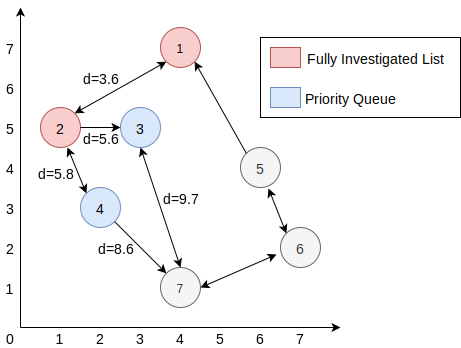
\includegraphics[height=5cm]{d.png}
\caption{Dijkstra's algorithm} \label{fig1}
\end{figure}

In regards to the cave problem described previously, Dijkstra's algorithm can be implemented in order to find the optimal route of any series of caves, or identify if no route is available. As the euclidean distance can be calculated using each points coordinates and a connectivity matrix is supplied, Dijkstra's algorithm will be able to start at cave one and work through every travereable neighbouring node until the last cave is reached.

% evaluation
Dijkstra's algorithm was first implemented on the ARMAC computer, which had only 15 kilobytes of memory, because of this small amount of memory, there were limitations in how advanced Dijkstra's shortest path first algorithm could be. The most major limitation in comparison to some of its successors was that it did not take into account any heuristic value for the nodes. Since only the distance travelled so far is taken into consideration and not the distance from the end node, the algorithm may first calculate nodes leading away from the end node before going back towards it.


% (13 Marks – maximum one page) Identify (don’t describe) a good algorithm to use for solving the problem and explain why it is good for this problem. 
\section{The A Star Pathfinding Algorithm}
Given the limitations of Dijkstra's algorithm, one of its successors, the A* search algorithm allows for an optimal route to be discovered much faster.  A* would be a more suitable choice of algorithm for the given problem of navigating a system of connected caves because it takes into consideration not only the distance travelled but a heuristic value as well. This heuristic value may be the euclidean distance or the Manhattan distance for example. By calculating the euclidean distance of each node (h(n)) and the distance travelled so far (g(n)), using the below formula (Fig 2) to determine which node to explore first provides an optimal solution at a much faster rate.




\begin{figure}
\begin{verbatim}
               f(n) = g(n) + h(n)
\end{verbatim}
\caption{ A* shortest-first algorithm} \label{fig1}
\end{figure}

% If the problem were to change so that the cost of taking a particular tunnel in a particular direction is given in the file – no-longer related to distance travelled, explain how this might affect your choice of algorithm and identify any problem that might occur in this situations.
In a situation where instead of using the euclidean distance as the distance travlled, each tunnel in a particular direction had a specified cost, the A* algorithm would not be the most suitable choice in finding an optimal path. In this scenario, the only given information to use when deciding which node to explore first is  g(n), no heuristic is available and therefor the formula shown in figure 1 is not usable.
Instead of using A* in this situation, Dijkstra's algorithm may be the more sensible implementation as it only requires a g(n) value.





\section{Conclusion}











% \figuremacro{h}{database}{Relational Database Structure}{ - User and Sound Tables}{1.0}

\noindent

\bibliographystyle{ieeetr}
\bibliography{references}

\clearpage
\section*{Appendices}	
\textbf{Appendix A}
	        
%	        \includegraphics[scale=0.6]{spotify}
%	        \textbf{Spotify Branding Guidlines} - Colour scheme and logo design (Spotify 2019)\cite{Spotify}


		
\end{document}